\documentclass[11pt,a4paper]{article}
\usepackage[margin=18mm]{geometry}
\usepackage{fontspec}
\usepackage{polyglossia}
\setdefaultlanguage{russian}
\setotherlanguage{english}
\setmainfont{Arial}
\setsansfont{Arial}
\setmonofont{Consolas}
\newfontfamily\cyrillicfont{Arial}[Script=Cyrillic]
\newfontfamily\cyrillicfontsf{Arial}[Script=Cyrillic]
\newfontfamily\cyrillicfonttt{Consolas}[Script=Cyrillic]
\usepackage{amsmath,amssymb,booktabs,tabularx,longtable}
\usepackage{graphicx,float,caption,microtype,xcolor,hyperref}
\graphicspath{{../results/figures/}}
\hypersetup{colorlinks=true,linkcolor=blue!50!black,urlcolor=blue!60!black}
\definecolor{accent}{HTML}{2563EB}
\definecolor{good}{HTML}{15803D}
\definecolor{warn}{HTML}{B45309}
\setlength{\parindent}{0pt}
\setlength{\parskip}{5pt}
\renewcommand{\arraystretch}{1.12}
% Generated from final CSV tables before release.
\newcommand{\MainResultShort}{KAN не ускоряет grokking универсально, а сдвигает границы между фазами обучения.}
\newcommand{\MainResultLong}{В полной матрице MLP дала 30/40 классических запусков, KAN --- 8/40. Локальный контраст возникает при $p=31$, 35\% train: MLP дала 0/10, KAN --- 8/10. При 50\% данных KAN обобщалась совместно или со слабой задержкой, а все 20 запусков $p=53$ получили класс weak delay.}
\newcommand{\KanFourierMem}{0.175}
\newcommand{\KanFourierGen}{0.828}
\newcommand{\KanFourierFinal}{0.952}
\newcommand{\MlpFourierMem}{0.075}
\newcommand{\MlpFourierFinal}{0.527}
\newcommand{\TopTenDelta}{-0.078}
\newcommand{\RandomTenDelta}{-0.047}
\newcommand{\BottomTenDelta}{0.000}
\newcommand{\RandomFourierFinal}{0.952}
\newcommand{\SymmetryFourierFinal}{0.165}
\newcommand{\PairedTableRows}{
KAN & 31 & 0.35 & 0.1 & 4/5 & 1 без обобщения & 4/5; 4.6k \\
KAN & 31 & 0.35 & 0.3 & 4/5 & 1 без обобщения & 4/5; 2.8k \\
KAN & 31 & 0.50 & 0.1 & 0/5 & weak 4, joint 1 & 5/5; 0.4k \\
KAN & 31 & 0.50 & 0.3 & 0/5 & weak 2, joint 3 & 5/5; 0.2k \\
KAN & 53 & 0.30 & 0.1 & 0/5 & weak 5 & 5/5; 3.9k \\
KAN & 53 & 0.30 & 0.3 & 0/5 & weak 5 & 5/5; 2.6k \\
KAN & 53 & 0.35 & 0.1 & 0/5 & weak 5 & 5/5; 2.3k \\
KAN & 53 & 0.35 & 0.3 & 0/5 & weak 5 & 5/5; 1.6k \\
MLP & 31 & 0.35 & 0.1 & 0/5 & 5 без обобщения & 0/5 \\
MLP & 31 & 0.35 & 0.3 & 0/5 & 5 без обобщения & 0/5 \\
MLP & 31 & 0.50 & 0.1 & 5/5 & -- & 5/5; 5.1k \\
MLP & 31 & 0.50 & 0.3 & 5/5 & -- & 5/5; 5.3k \\
MLP & 53 & 0.30 & 0.1 & 5/5 & -- & 5/5; 10.3k \\
MLP & 53 & 0.30 & 0.3 & 5/5 & -- & 5/5; 13.4k \\
MLP & 53 & 0.35 & 0.1 & 5/5 & -- & 5/5; 6.2k \\
MLP & 53 & 0.35 & 0.3 & 5/5 & -- & 5/5; 7.2k \\
}


\begin{document}

\begin{titlepage}
\vspace*{24mm}
{\color{accent}\large Самостоятельная исследовательская работа\par}
\vspace{12mm}
{\Huge\bfseries Grokking модульной арифметики:\par}
\vspace{3mm}
{\LARGE\bfseries парное сравнение quadratic MLP и spline-KAN\par}
\vspace{14mm}
{\large Научный отчёт\par}
\vspace{4mm}
{\large Автор: Варфоломеев Матвей Денисович\par}
\vfill
\begin{tabular}{@{}ll@{}}
Задача & $y=(a+b)\bmod p$ \\
Основная серия & 80 запусков, seed 10--14 \\
Архитектуры & quadratic MLP на основе Громова и spline-KAN \\
Среда & Python 3.12, PyTorch 2.7.1 \\
Год & 2026
\end{tabular}
\vspace{12mm}

\textbf{Краткий результат.} \MainResultShort
\end{titlepage}

\section{Аннотация и исследовательский вопрос}

Grokking --- это позднее обобщение после раннего запоминания и долгого плато.
Работа проверяет, как эта последовательность меняется при замене минимальной
quadratic MLP на основе архитектуры Громова на spline-KAN сопоставимого
размера. One-hot данные, MSE, full-batch AdamW и seed общие. После
exploratory-поиска зафиксирована подтверждающая матрица из 80 запусков:
модули 31 и 53, четыре сочетания модуля и доли данных, две архитектуры и два
weight decay. В статистику входят все кривые.

\textbf{Главный вывод.} \MainResultLong

KAN не объявляется лучшей архитектурой, а высокая точность --- пониманием
арифметики. Вывод ограничен исследованными моделями, split и бюджетом.

\section{Контекст и литература}

Power et al. описали позднее обобщение на малых алгоритмических датасетах;
Nanda et al. связали скачок test accuracy с постепенной Fourier-динамикой.
Gromov предложил минимальную bias-free quadratic MLP с MSE и аналитическими
feature maps для модульной арифметики. Park et al. используют
Kolmogorov--Arnold representation для переноса весов в transformer, но это не
реализованный здесь spline-KAN.

KAN заменяет вес ребра обучаемой одномерной функцией. Это контролируемое
вмешательство: меняется вычислительный блок, данные и критерий фаз --- нет.

\textbf{Разделение частей работы:}

\begin{itemize}
  \item архитектурная основа -- bias-free quadratic MLP, one-hot и MSE из
        постановки Громова;
  \item адаптация -- общий full-batch AdamW для контролируемого сравнения;
  \item расширение -- парный spline-KAN и многосидовый механистический анализ.
\end{itemize}

\clearpage
\section{Данные, модели и функция потерь}

Для простого $p$ используются все $p^2$ пар $(a,b)\in\mathbb Z_p^2$. Вход
имеет вид
\[
x=[\operatorname{onehot}(a),\operatorname{onehot}(b)]\in\mathbb R^{2p},
\qquad
y=\operatorname{onehot}((a+b)\bmod p)\in\mathbb R^p.
\]
Основная серия использует случайный split; фактическая доля train сохраняется,
поскольку число примеров целое.

\subsection{Quadratic MLP}

MLP не содержит bias. Для ширины $h=128$:
\[
f(x)=\frac{1}{h}W_2\left(\frac{W_1x}{\sqrt{2p}}\right)^{\!2}.
\]
Нормировки, отсутствие bias и активация следуют архитектуре Громова. Его
точный gradient-descent протокол здесь не воспроизводится: оптимизатор основной
матрицы --- AdamW.

\subsection{Spline-KAN}

KAN имеет два слоя и ширину 14. Каждое направленное ребро вычисляет
\[
\phi(x)=w_{\mathrm{base}}\operatorname{SiLU}(x)+
\sum_k w_k B_k(x),
\]
где $B_k$ --- фиксированные кубические B-spline basis functions; оба набора
коэффициентов обучаются. При \texttt{grid\_size=5} и
\texttt{spline\_order=3} числа параметров MLP/KAN равны 11,904/11,718 для
$p=31$ и 20,352/20,034 для $p=53$.

\subsection{Оптимизация}

Loss --- средний квадрат расстояния до one-hot цели:
\[
\mathcal L=\frac1N\sum_{i=1}^{N}\|f(x_i)-y_i\|_2^2.
\]
Парные запуски используют full-batch AdamW, learning rate 0.001, weight decay
0.1 или 0.3 и обучение без досрочной остановки.

\clearpage
\section{Строгий критерий grokking и протокол}

Сначала exploratory-этап проверял $p=97$ и помог уточнить постановку. Затем, до
просмотра результатов новой серии, были зафиксированы критерий ниже, матрица и
seed. Поэтому подтверждающей является серия из 80 запусков, а не весь проект.

99\% test accuracy недостаточно. Метка \texttt{classical\_grokking} требует:

\begin{enumerate}
  \item train accuracy не ниже 0.99 на пяти последовательных измерениях;
  \item test accuracy в начале устойчивого запоминания не выше 0.20;
  \item разрыв train--test в этой точке не меньше 0.50;
  \item до достижения 0.90 test accuracy проходит не менее 1000 шагов;
  \item затем test accuracy устойчиво достигает 0.99.
\end{enumerate}

Другие классы: слабая задержка, совместное обобщение, запоминание без обобщения
и отсутствие запоминания. Незавершившийся запуск цензурируется, но остаётся в
знаменателе.

\begin{table}[H]
\centering
\caption{Подтверждающая матрица, зафиксированная после exploratory-этапа.}
\begin{tabular}{@{}llll@{}}
\toprule
Модуль и train & Бюджет & Модели & Weight decay \\
\midrule
$p=31$, 35\% & 15,000 & MLP, KAN & 0.1, 0.3 \\
$p=31$, 50\% & 15,000 & MLP, KAN & 0.1, 0.3 \\
$p=53$, 30\% & 20,000 & MLP, KAN & 0.1, 0.3 \\
$p=53$, 35\% & 20,000 & MLP, KAN & 0.1, 0.3 \\
\bottomrule
\end{tabular}
\end{table}

Каждая ячейка использует seed 10--14 и измерения раз в 100 шагов. Для фаз
приводится Wilson 95\% interval; для задержки --- медиана, диапазон и число
обобщившихся запусков.

\begin{figure}[H]
\centering
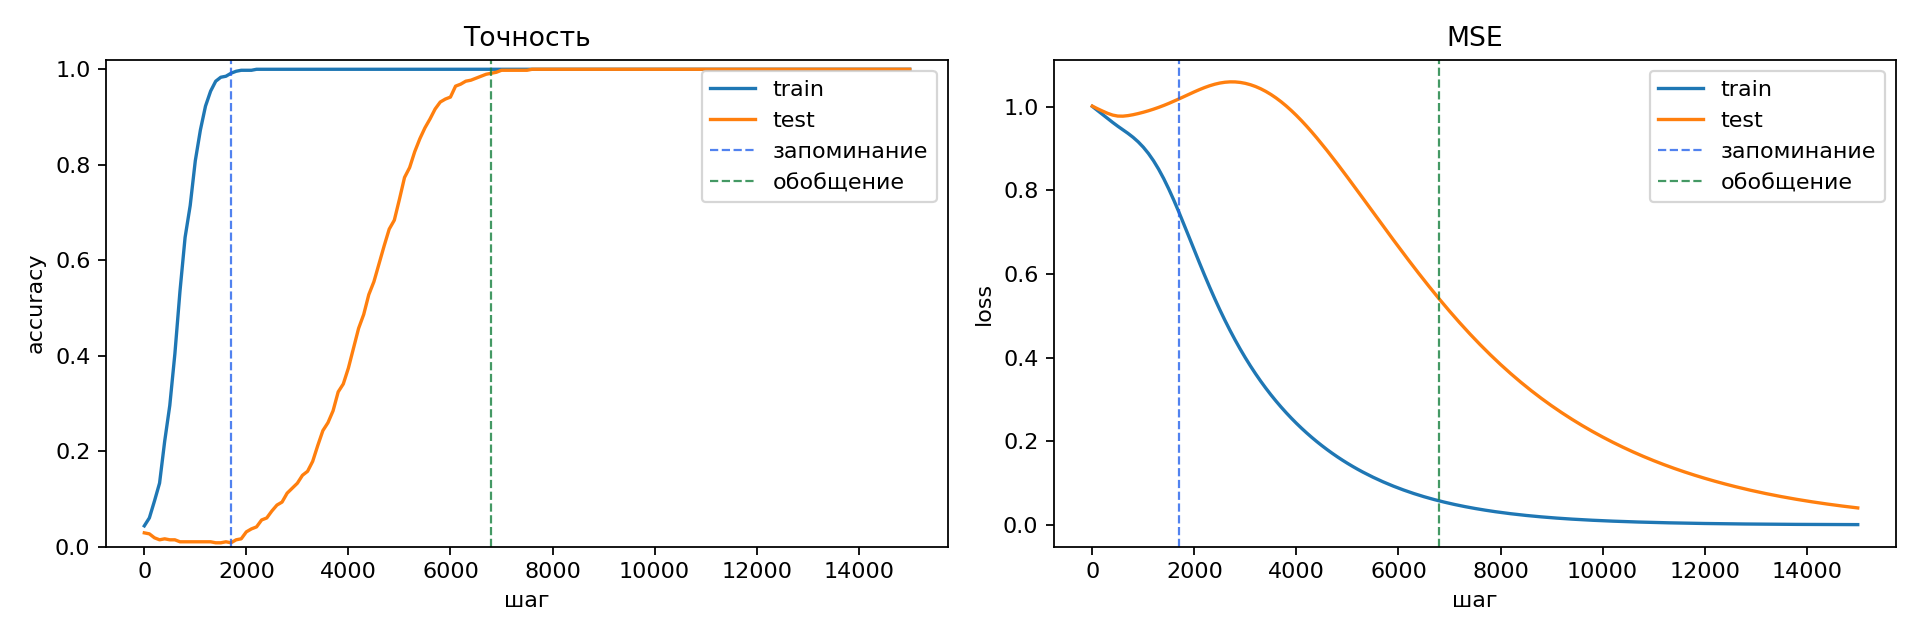
\includegraphics[width=\textwidth]{example_classical_mlp/learning_curves.png}
\caption{Пример классического grokking в новой серии: MLP, $p=31$, 50\%,
\texttt{wd=0.1}, seed 10.}
\end{figure}

\clearpage
\section{Парная фазовая карта}

\begin{figure}[H]
\centering
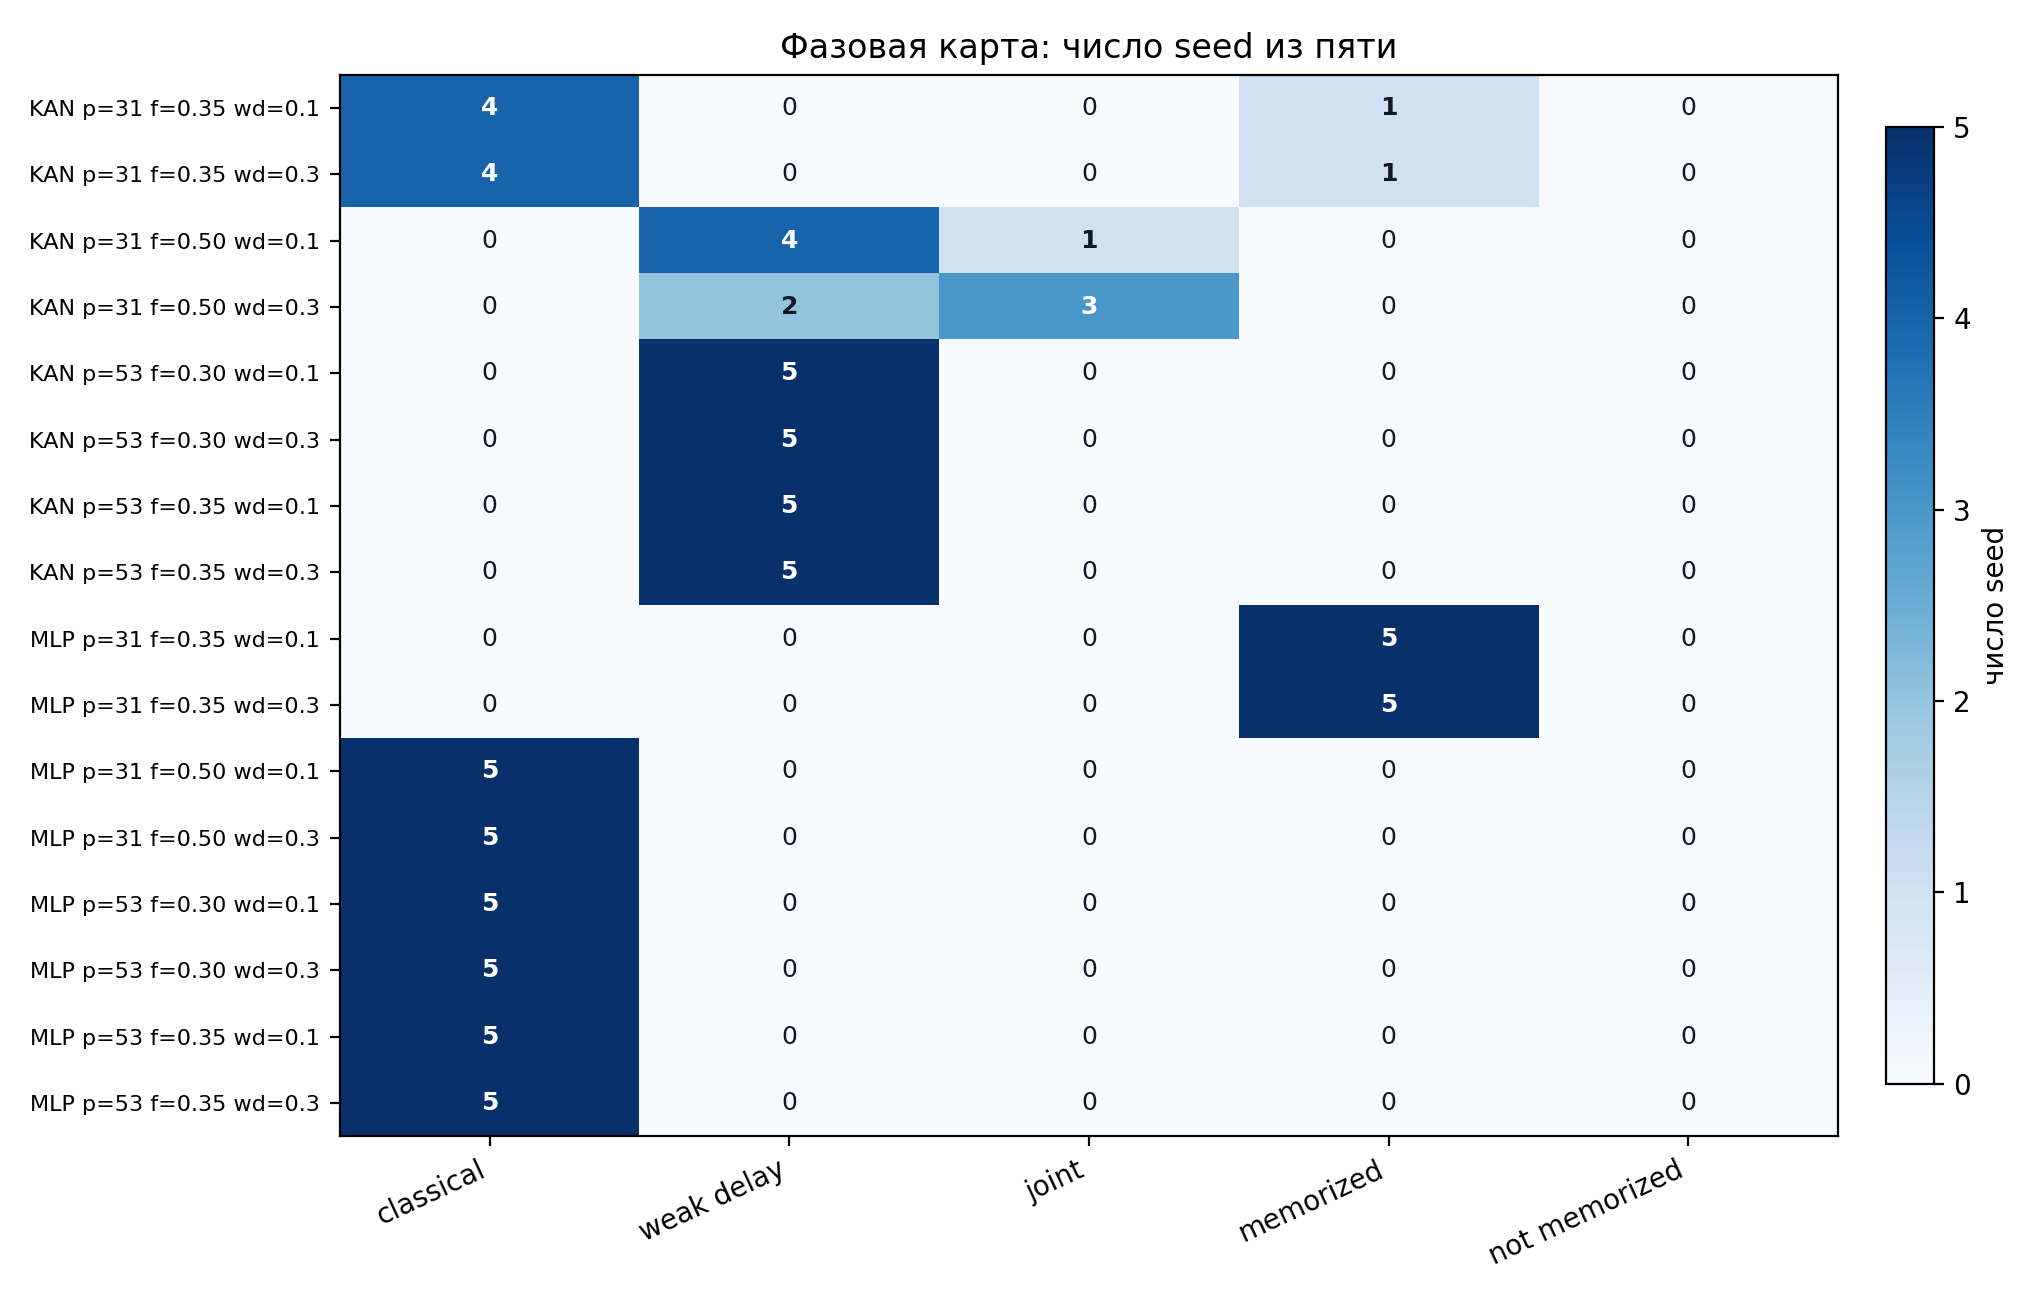
\includegraphics[width=0.94\textwidth]{paired_phase_heatmap.png}
\caption{Все пять seed каждой ячейки классифицированы одним и тем же
критерием.}
\end{figure}

\begin{table}[H]
\centering
\small
\caption{Сжатая сводка фаз. Полные Wilson intervals находятся в
\texttt{results/tables/paired\_summary.csv}.}
\begin{tabular}{@{}llrrlll@{}}
\toprule
Модель & $p$ & Train & WD & Classical & Другие фазы & Обобщились \\
\midrule
\PairedTableRows
\bottomrule
\end{tabular}
\end{table}

Главной является эта таблица, а не исторические удачные кривые. Сравнение
парное по $p$, train и weight decay и не переносится на другие модели или
задачи. Wilson 95\% intervals равны 0.376--0.964 для 4/5 и 0.566--1.000 для
5/5: повторяемость видна, но оценка вероятности широка.

\clearpage
\section{Задержка и цензурирование}

\begin{figure}[H]
\centering
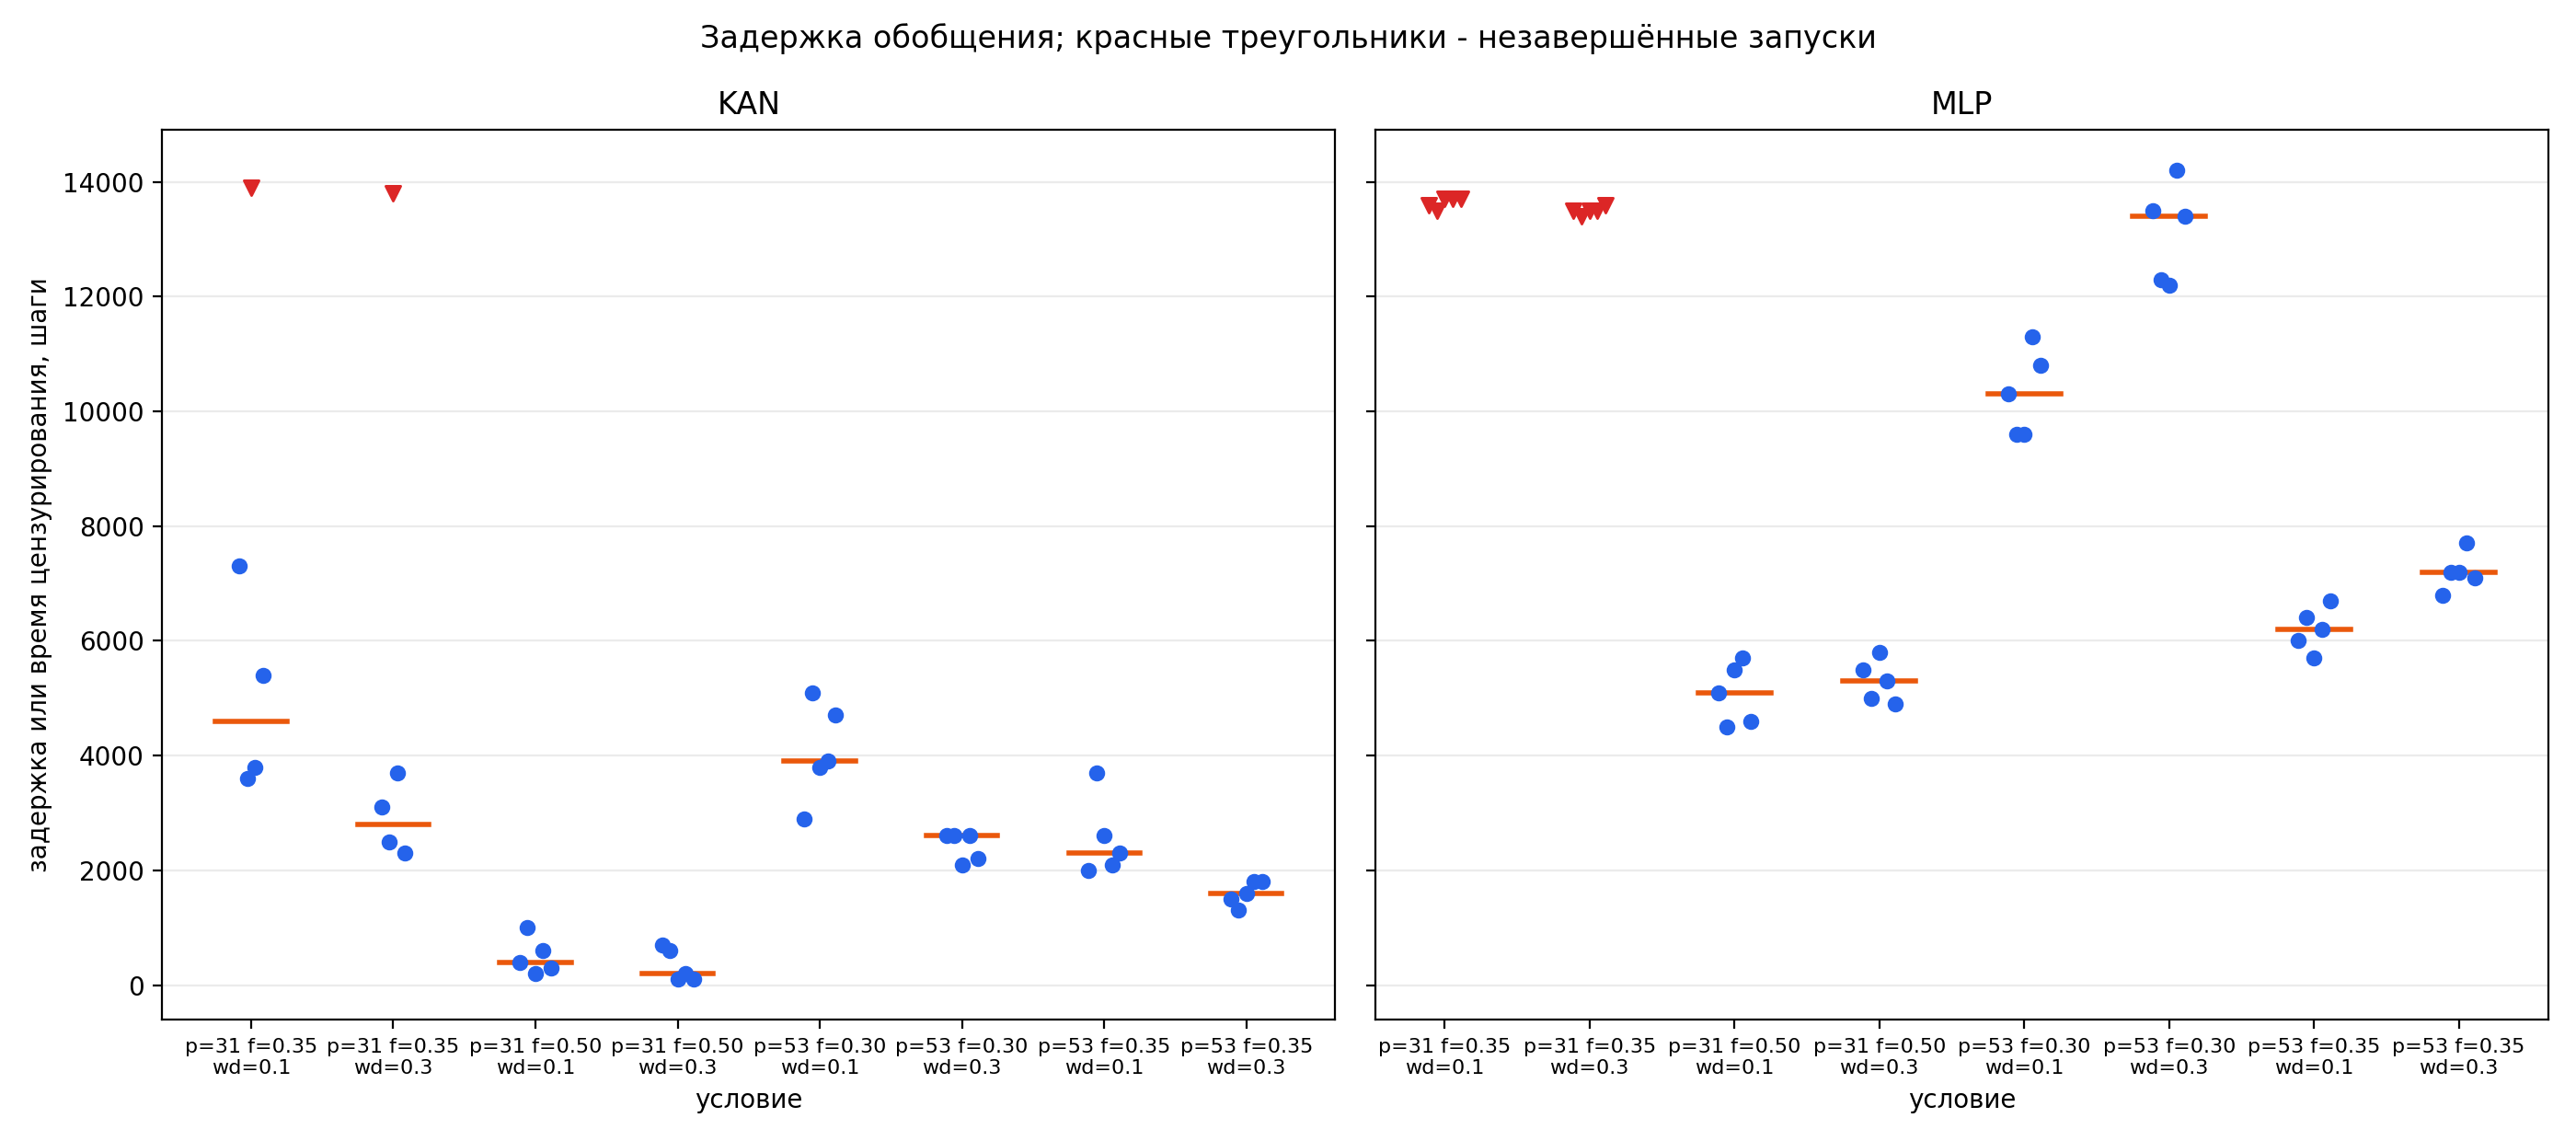
\includegraphics[width=\textwidth]{paired_delays.png}
\caption{Точки -- отдельные seed, оранжевая линия -- медиана наблюдавшихся
задержек, красные треугольники -- правое цензурирование.}
\end{figure}

Задержка идёт от устойчивого train-запоминания до устойчивого test-обобщения.
Если обобщение не наступило, время наблюдения показывается как цензурированное
и не входит в медиану, поэтому модели с меньшим числом успешных seed не получают
искусственного преимущества.

\section{Многосидовая Fourier- и PCA-динамика}

Для $p=31$, 35\% train, \texttt{wd=0.3} сохранены состояния запоминания,
обобщения и финала. Логиты каждого класса образуют таблицу $p\times p$;
двумерный FFT измеряет долю мощности на $f_a=f_b$ без DC-компоненты.

\begin{figure}[H]
\centering
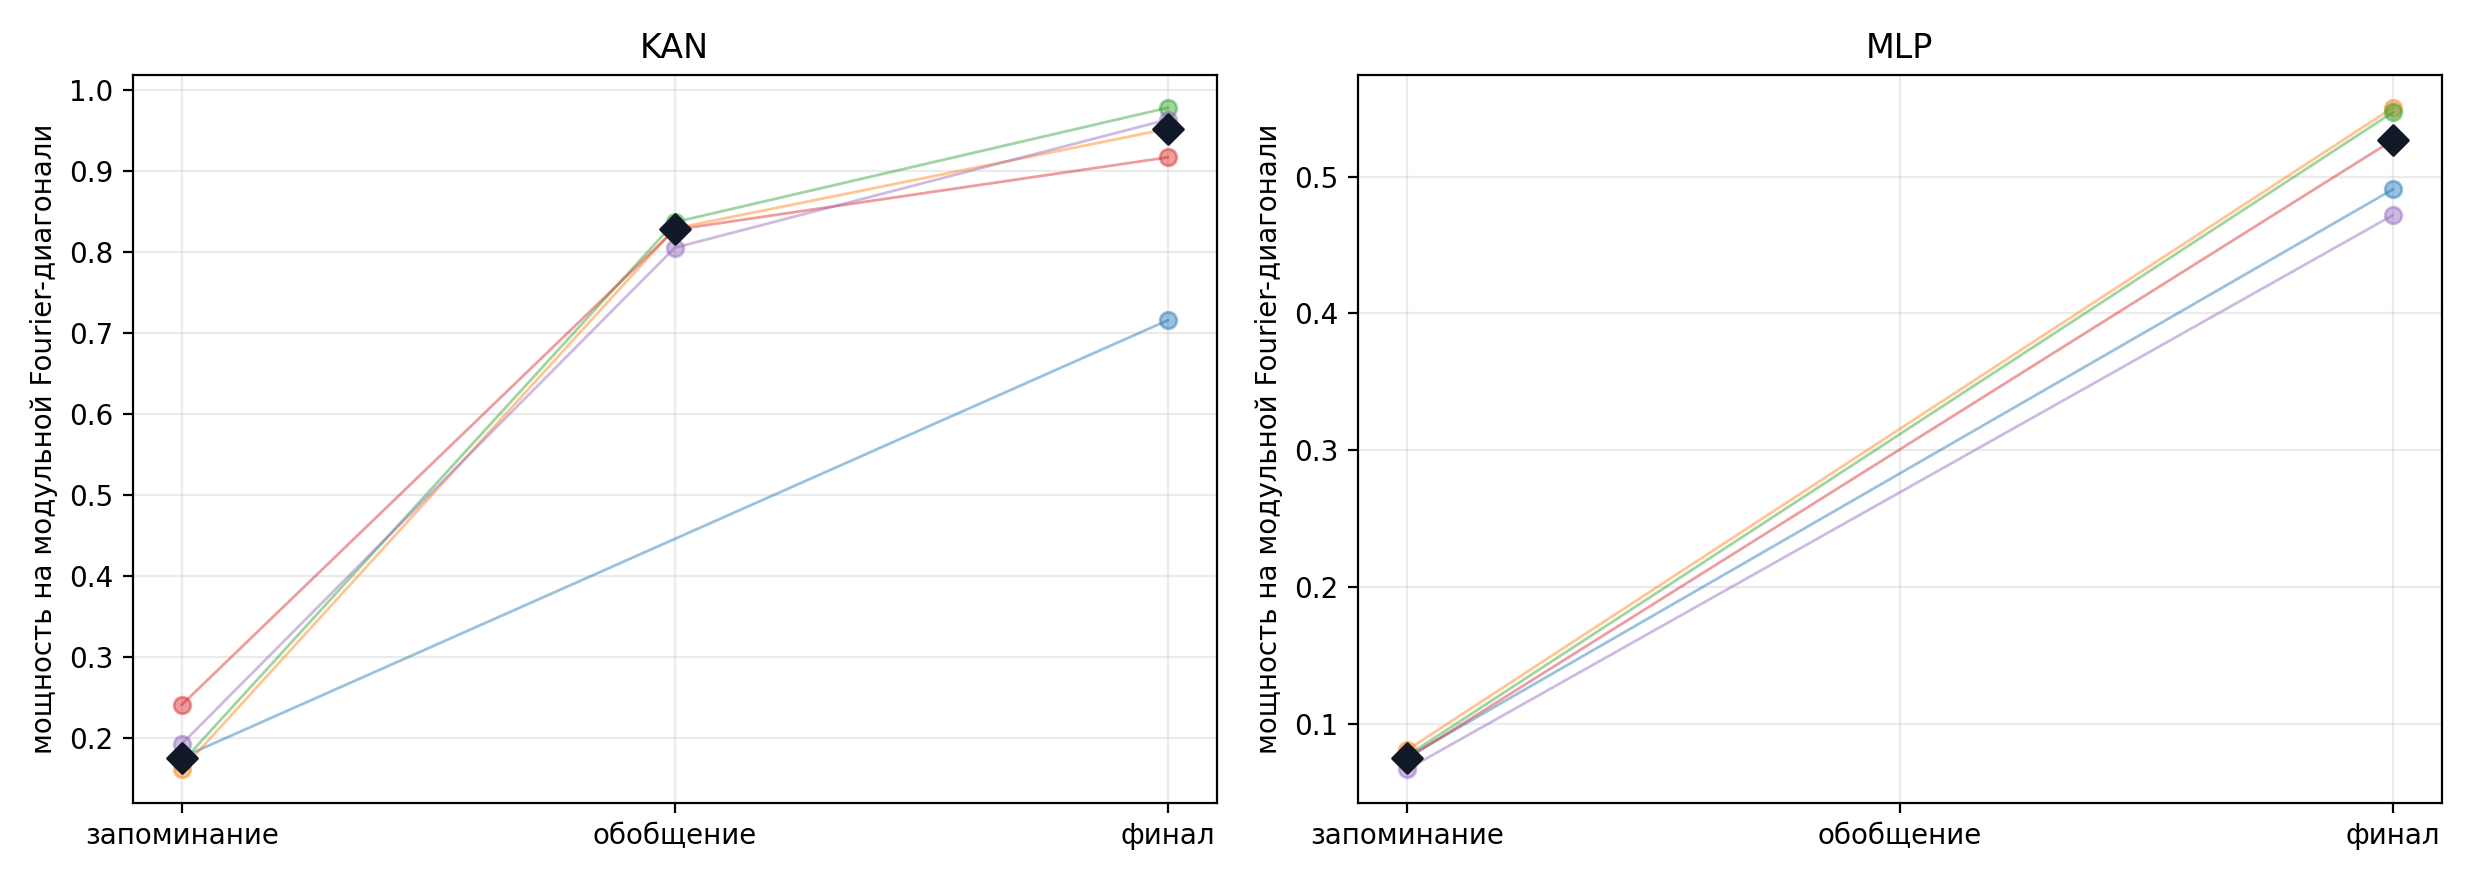
\includegraphics[width=0.84\textwidth]{fourier_multiseed.png}
\caption{Fourier-динамика всех доступных фаз. У MLP в этом условии точка
обобщения отсутствует, поскольку пять запусков цензурированы.}
\end{figure}

Медиана KAN растёт с \KanFourierMem{} при запоминании до \KanFourierGen{} при
обобщении четырёх seed и \KanFourierFinal{} в финале. У MLP она растёт с
\MlpFourierMem{} до \MlpFourierFinal{} без строгого test-порога. Поэтому
Fourier-концентрация --- progress measure, а не критерий grokking. Participation
rank, эффективное число направлений дисперсии скрытого слоя, меняется
неодинаково между seed и служит только диагностикой.

Полный средний classwise-спектр сохранён для каждой пары частот
$(f_a,f_b)$, каждого seed и checkpoint. Ведущие моды вынесены в отдельную
таблицу; это позволяет проверить волновую структуру, а не только один
диагональный показатель.

\begin{figure}[H]
\centering
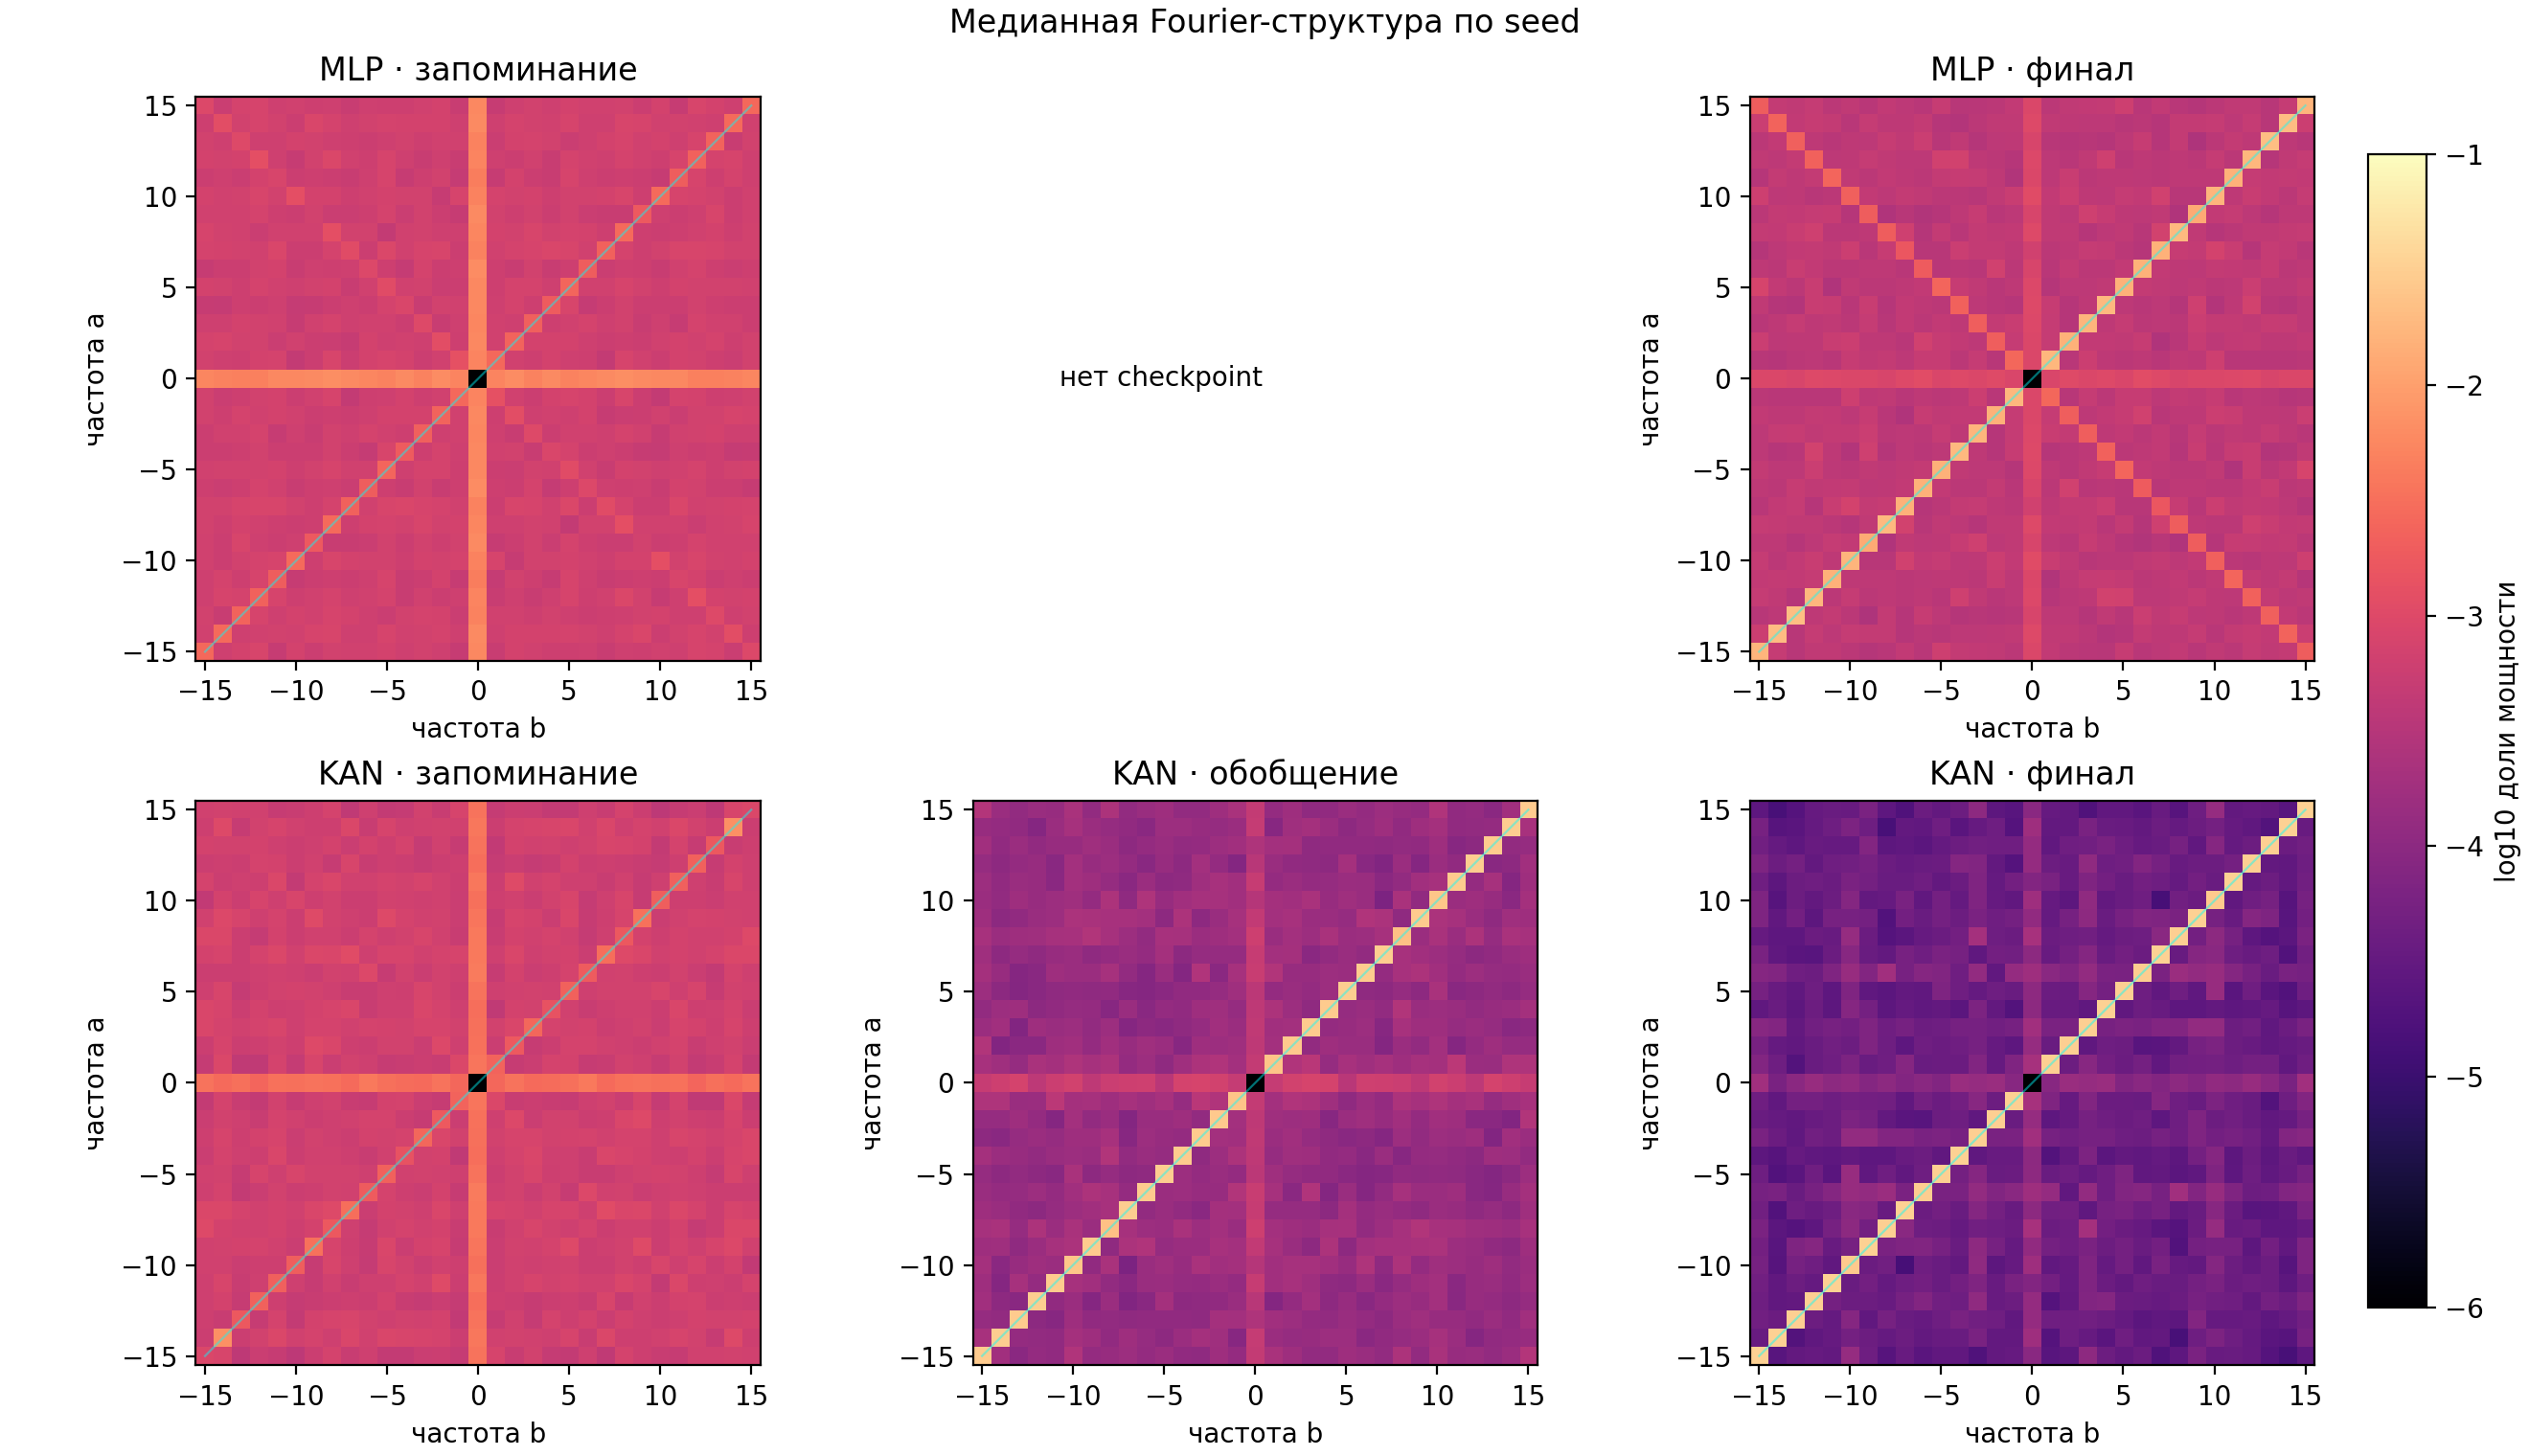
\includegraphics[width=0.94\textwidth]{fourier_spectrum_heatmaps.png}
\caption{Медианный по seed полный Fourier-спектр. Голубая линия показывает
модульную диагональ $f_a=f_b$; отсутствие MLP-checkpoint обобщения оставлено
явным.}
\end{figure}

\clearpage
\section{Edge-ablation и проверка переноса}

Важность KAN-ребра --- RMS его вклада на всех $p^2$ входах. Для top, random или
bottom рёбер вместе зануляются base- и spline-коэффициенты; random повторяется
десять раз на модель.

\begin{figure}[H]
\centering
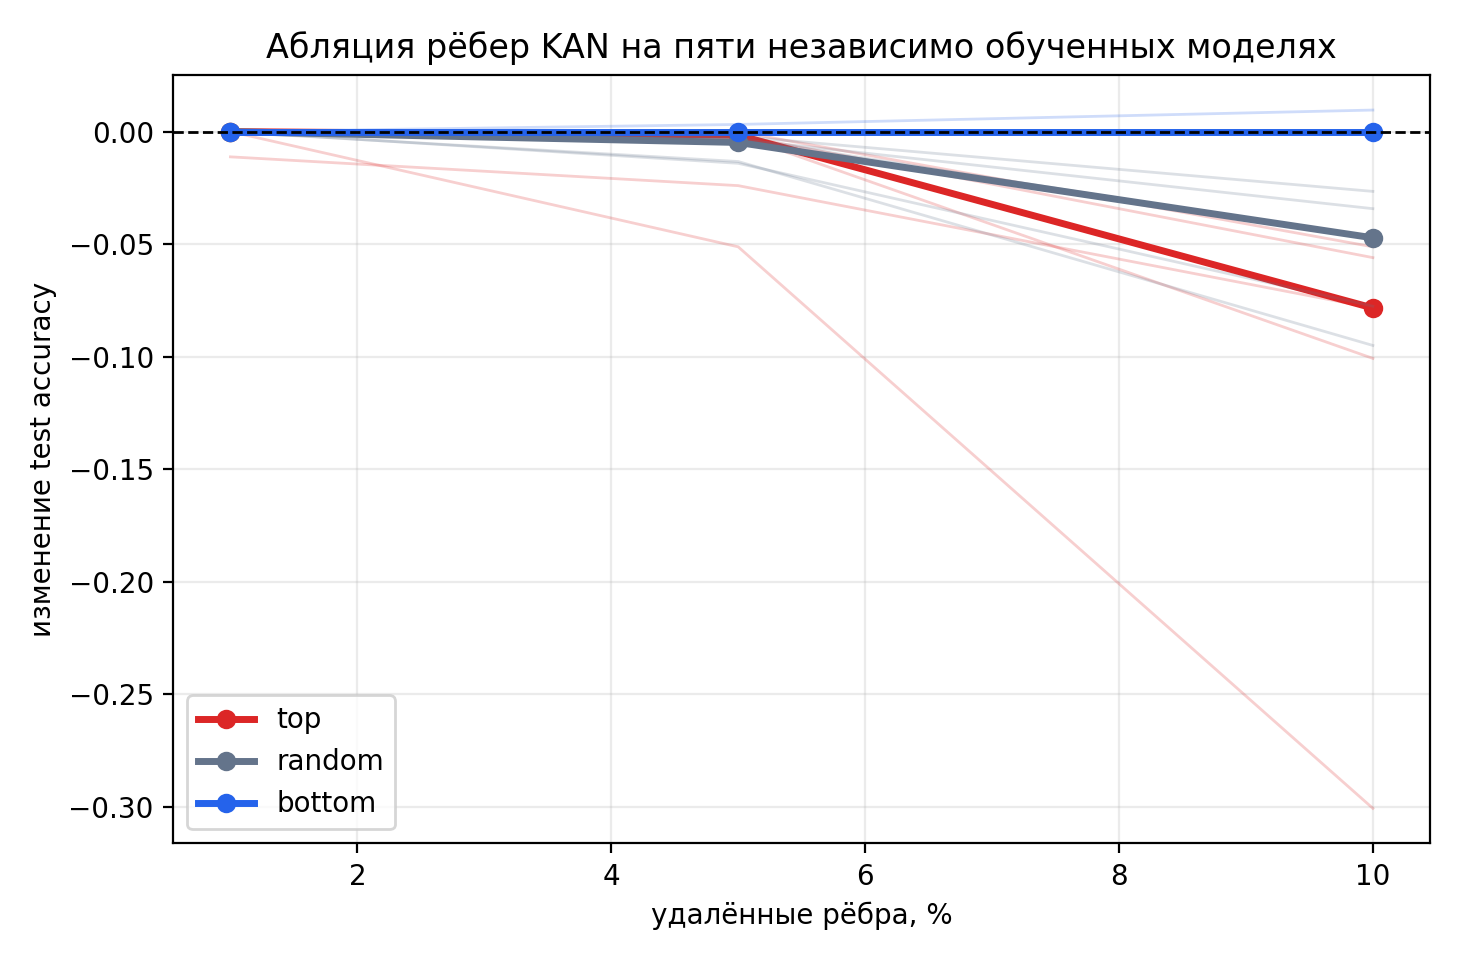
\includegraphics[width=0.82\textwidth]{edge_ablation_multiseed.png}
\caption{Изменение test accuracy относительно baseline для пяти KAN. Тонкие
линии -- seed, толстые -- медиана.}
\end{figure}

Удаление 10\% рёбер меняет test accuracy на \TopTenDelta{} для top,
\RandomTenDelta{} для random и \BottomTenDelta{} для bottom. Top сильнее bottom
в 5/5 моделей, но сильнее random-медианы в 4/5: концентрация относительно
bottom устойчива, утверждение ``top всегда важнее random'' --- нет.

Symmetry-safe split проверяет перенос через коммутативность. В успешном
random-split режиме KAN получила 8/10 classical grokking, но на symmetry-safe
split --- 0/5. MLP при $p=31$, 50\% сохранила 5/5. Поэтому результат KAN
чувствителен к структуре разбиения. Финальные медианы Fourier-концентрации:
\RandomFourierFinal{} для random и \SymmetryFourierFinal{} для symmetry-safe.
Плохое обобщение symmetry-safe KAN не позволяет трактовать их абляции как
механизм успешного решения.

\begin{figure}[H]
\centering
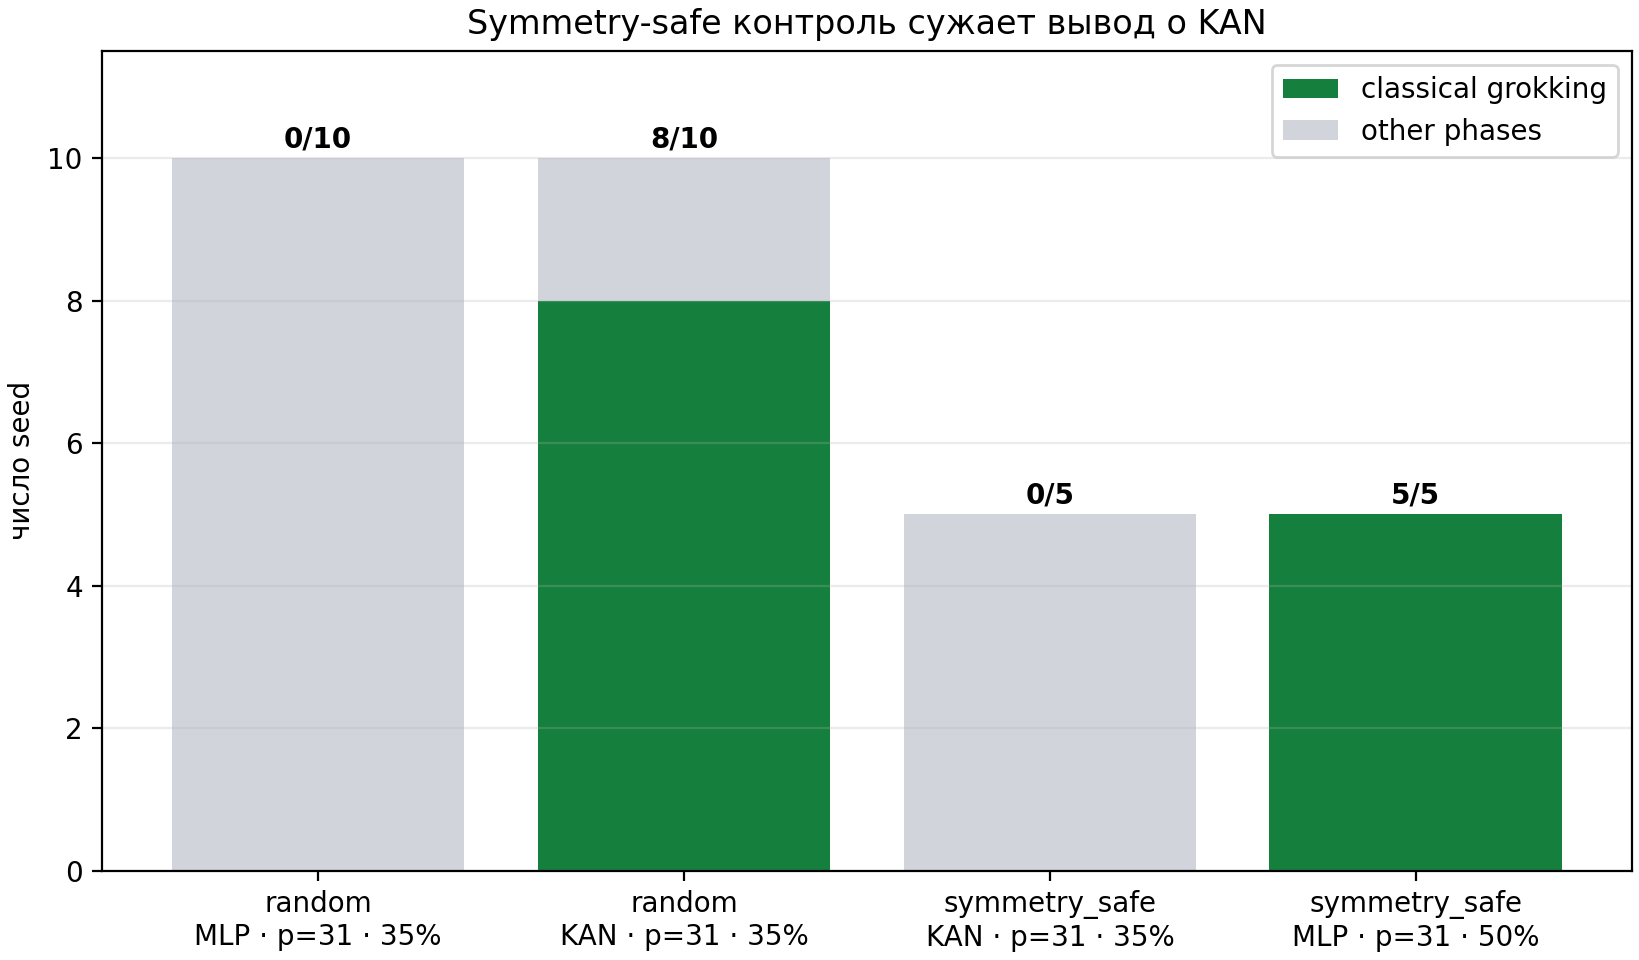
\includegraphics[width=0.82\textwidth]{symmetry_phase_comparison.png}
\caption{Полные знаменатели random и symmetry-safe контролей. Условия MLP и
KAN в symmetry-safe части различаются по train fraction и не образуют прямую
парную ячейку; график проверяет устойчивость заявленных успешных режимов.}
\end{figure}

\clearpage
\section{Ограничения, изменение гипотезы и вывод}

\subsection*{Как менялась гипотеза}

Exploratory-режим $p=97$ не показал длинного плато: модель либо обобщала сразу,
либо не проходила нужные фазы. После этого подтверждающая серия была
зафиксирована на 31 и 53, порог 99\% заменён строгой классификацией, а
symmetry-safe контроль выявил зависимость эффекта от split.

\subsection*{Ограничения}

\begin{itemize}
  \item Сравниваются две конкретные ширины и один B-spline basis.
  \item Пять seed проверяют повторяемость, но широкие Wilson intervals не дают
        сильных популяционных выводов.
  \item AdamW делает сравнение контролируемым, но отделяет его от точного
        gradient-descent протокола Громова.
  \item One-hot вход ограничивает интерпретацию непрерывной формы KAN-ребра:
        первый слой наблюдает главным образом значения 0 и 1.
  \item Fourier-концентрация согласуется с модульной структурой, но не
        доказывает единственный внутренний алгоритм.
\end{itemize}

\subsection*{Вывод}

Получена воспроизводимая карта фаз, а не рейтинг архитектур; сохранены все seed
и отрицательные результаты. На random split KAN входит в classical grokking
при меньшей доле данных, но symmetry-safe контроль показывает чувствительность
этого эффекта к разбиению. Fourier и ablation дают поддерживающие свидетельства,
а не доказательство единственного алгоритма.

\section*{Литература}

\small
\begin{enumerate}
  \item Power, A. et al. \emph{Grokking: Generalization Beyond Overfitting on
        Small Algorithmic Datasets}. arXiv:2201.02177, 2022.
  \item Gromov, A. \emph{Grokking modular arithmetic}. arXiv:2301.02679, 2023.
  \item Nanda, N. et al. \emph{Progress measures for grokking via mechanistic
        interpretability}. arXiv:2301.05217, 2023.
  \item Liu, Z. et al. \emph{KAN: Kolmogorov-Arnold Networks}.
        arXiv:2404.19756, 2024.
  \item Park, Y.; Kim, M.; Kim, Y. \emph{Acceleration of Grokking in Learning
        Arithmetic Operations via Kolmogorov-Arnold Representation}.
        \emph{Neurocomputing} 640 (2025), 130347.
        DOI: 10.1016/j.neucom.2025.130347.
\end{enumerate}

\end{document}
